\documentclass[border=2mm]{standalone}
\usepackage{xcolor}
\usepackage{pgfplots}
\usepackage{tikz}
\usetikzlibrary{patterns}

% Define bar chart colors
\definecolor{bblue}{HTML}{4F81BD}
\definecolor{rred}{HTML}{C0504D}
\definecolor{ggreen}{HTML}{9BBB59}
\definecolor{ppurple}{HTML}{9F4C7C}


\begin{document}
	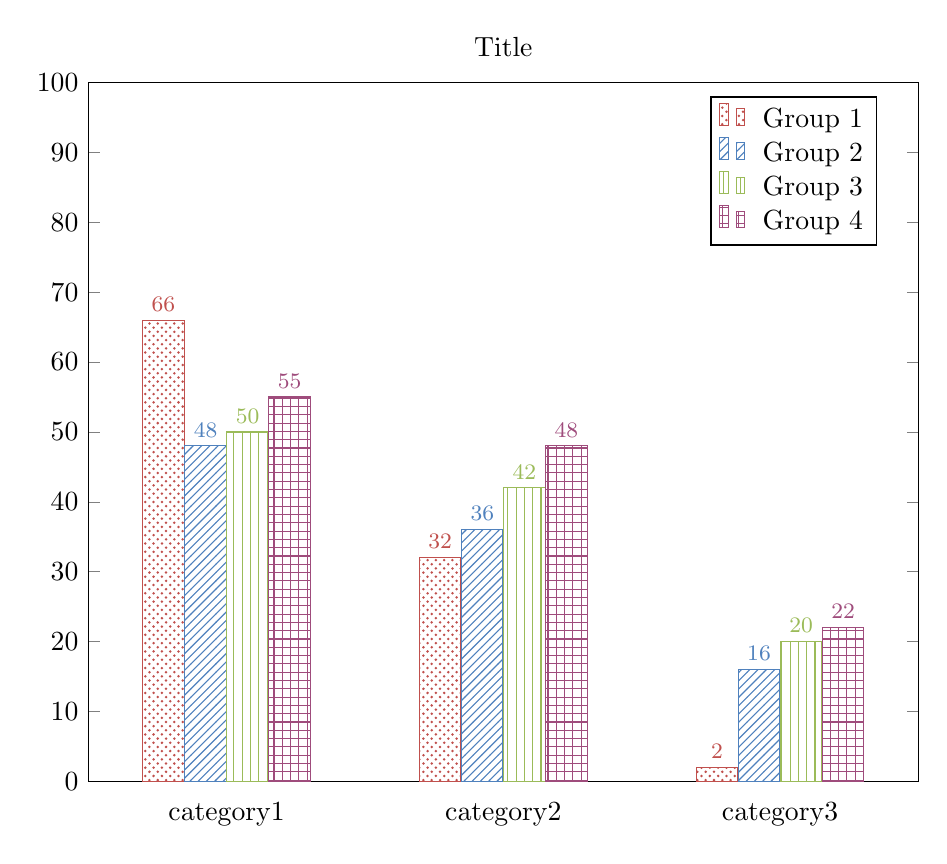
\begin{tikzpicture}
	    \begin{axis}[	
		title={Title},
		width  = \textwidth,
%		height = 6cm,
		major x tick style = transparent,
		%TODO category names
		symbolic x coords={category1, category2, category3},
		xtick = data,
		enlarge x limits=0.25,
		scaled y ticks = false,
		ymin=0,
		ymax=100,
		ybar=0.5\pgflinewidth,
		bar width=15pt,
%		ymajorgrids = true,
%		ylabel = {\%},
		nodes near coords,
		nodes near coords align={vertical},
		every node near coord/.append style={font=\footnotesize, inner sep=3pt},
		legend cell align=center,
		legend style={
		        at={(0.85,0.98)},
		        anchor=north,
		        column sep=1ex
		}
	    ]

		%TODO category names
		\addplot[rred,style={postaction={pattern color=rred,pattern=crosshatch dots}}]
			 coordinates {(category1,66) (category2,32) (category3,2)};
		\addplot[bblue,style={ postaction={pattern color=bblue,pattern=north east lines}}]
			coordinates {(category1,48) (category2,36) (category3,16)};
		\addplot[ggreen,style={ postaction={pattern color=ggreen,pattern=vertical lines}}]
			coordinates {(category1,50) (category2,42) (category3,20)};			
		\addplot[ppurple,style={ postaction={pattern color=ppurple,pattern=grid}}]
			coordinates {(category1,55) (category2,48) (category3,22)};
				
		%TODO Group names names		
		\legend{Group 1,Group 2,Group 3,Group 4}
	    \end{axis}
	\end{tikzpicture}
\end{document}
